%%%%%%%%%%%%%%%%%%%%%%%%%%%%%%%%%%%%%%%%%%%%%%%%%%%%%%%%%%%%%%%%%%%%%%%%%%%%%%%%
\section{Considerações Iniciais}

Os resultados encontrados ao rebalancear classes a partir da geração de imagens artificiais estão descritos neste capítulo. Para cada experimento realizado, são descritos: o protocolo utilizado (incluindo a base de imagens e os métodos de conversão para escala de cinza e extração de características), os resultados encontrados e a discussão da relevância de tais resultados.

Foram realizados diversos experimentos direcionados a explorar o rebalanceamento com métodos de processamento, para melhorar a acurácia da classificação de bases de imagens. Como entrada são utilizadas imagens originais provenientes de diversas coleções disponíveis na literatura. Como resultado, são calculadas medidas estatísticas da classificação dessas coleções após a alteração dessas imagens com os métodos de realce de características relevantes.

Os experimentos a serem relatados são relacionados à geração de imagens para rebalancear classes. Tal processamento é realizado antes da extração de características, e portanto no campo visual. Por conta disso, os resultados devem refletir melhoras nas etapa subsequente de classificação.

%%%%%%%%%%%%%%%%%%%%%%%%%%%%%%%%%%%%%%%%%%%%%%%%%%%%%%%%%%%%%%%%%%%%%%%%%%%%%%%%

\section{Experimentos}

Esta seção descreve os resultados encontrados ao rebalancear as classes de imagens aplicando os processamentos --- descritos no Capítulo \ref{cap:metodo} --- nas imagens originais. A Figura \ref{fig:fluxo} destaca o fluxo de operações realizadas para a análise do impacto da geração de imagens no rebalanceamento de classes. O mesmo protocolo de conversão para escala de cinza, extração de características e classificação foi seguido para três sub-experimentos: base desbalanceada; base rebalanceada com interpolação dos vetores de características (método SMOTE); e base rebalanceada com a geração artificial de imagens.

\begin{figure}[!htbp]
\centering
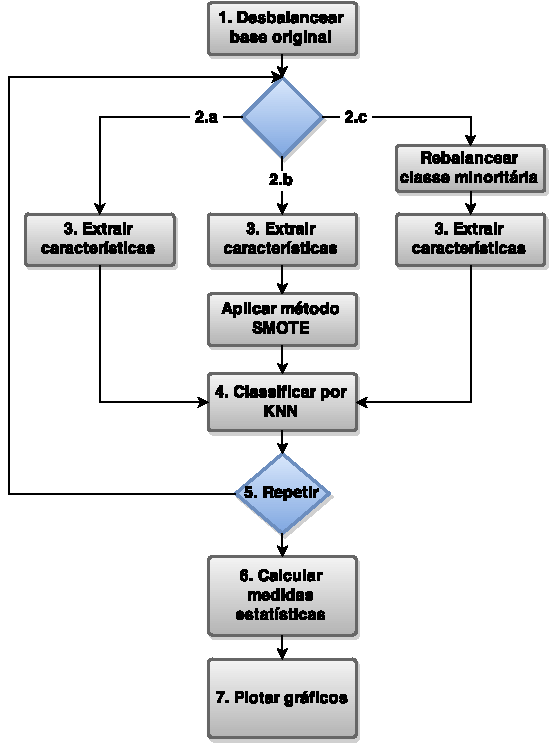
\includegraphics[scale=1.1]{\detokenize{figuras/flow_main.pdf}}
\caption[Fluxo de operações para obtenção dos resultados do rebalanceamento de classes]{Fluxo de operações para obtenção dos resultados do rebalanceamento de classes. \textit{Fonte:~Elaborado pela autora.}}
\label{fig:fluxo}
\end{figure}

Procurando estabilidade dos resultados obtidos com a geração das imagens artificiais, foi identificada a necessidade de controlar a remoção de imagens da base no momento da criação da base desbalanceada. Assim, os resultados foram obtidos a partir de uma forma de validação K-fold com o objetivo de prover mais robustez ao sistema. A Figura \ref{fig:folds} ilustra como tal validação foi realizada, utilizando como exemplo uma base com duas classes de imagens. Primeiramente as imagens foram separadas de forma aleatória em $k=5$ folds em cada classe. Depois, as duas classes compõem 40 configurações, consistindo em: um fold para teste e os outros para treino na classe que permanecerá balanceada; e um de teste e um de treino para a classe que os métodos de processamento irão rebalancear. Tal validação é repetido para todas as classes, ou seja, cada classe contribui para o desbalanceamento. Porém, se originalmente a base é naturalmente desbalanceada, um fold é utilizado para teste e os restantes para treino para todas as classes.

\begin{figure}[!htbp]
\centering
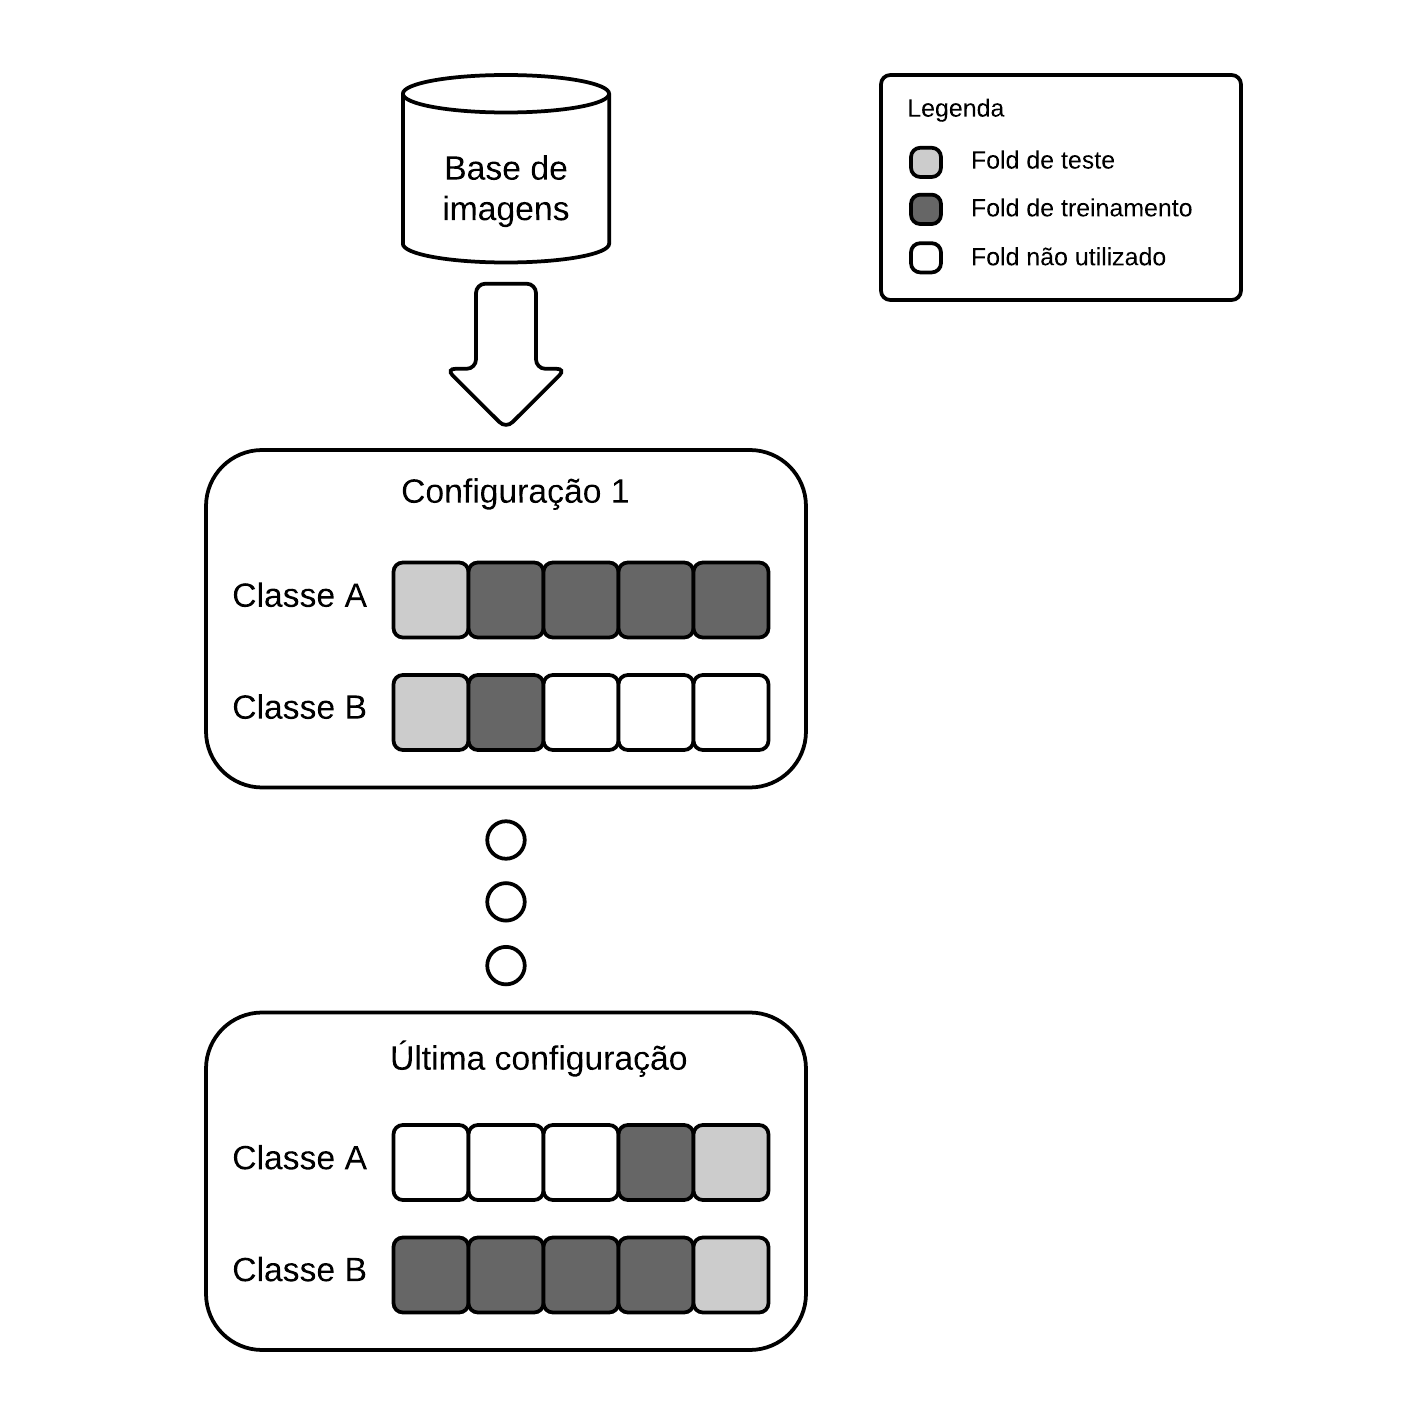
\includegraphics[scale=0.3]{\detokenize{figuras/folds_chart.png}}
\caption[]{\textit{Fonte:~Elaborado pela autora.}}
\label{fig:folds}
\end{figure}

A medida estatística mais comum para avaliação é a razão do número de acertos pela quantidade de imagens testadas. Essa medida, conhecida por \underline{acurácia}, pode não refletir propriamente os resultados, em um cenário de bases desbalanceadas. Isso se deve ao fato de que se a classe minoritária não obtiver nenhum resultado correto e a classe majoritária tiver 100\% de acertos, a acurária normal poderá ser muito alta, mesmo considerando que nenhuma imagem da classe minoritária foi corretamente classificada. Dessa forma, considera que os erros são igualmente importantes. Mas em se tratando de bases desbalanceadas, deve-se diferenciar o erro em, por exemplo, diagnosticar um paciente doente -- classe minoritária -- como sendo saudável e um paciente saudável -- classe majoritária -- como estando doente \cite{Batista2004}. No primeiro caso, o paciente corre risco de diagnóstico tardil, enquanto o paciente saudável realiza outros testes para refutação.

Pode-se estender essa medida obtendo-se a \underline{acurácia $k$-fold}: medida de acerto baseada na divisão do conjunto de objetos em teste e treinamento, realizando a repetição dos experimentos $n$ vezes e obtendo a média e o desvio padrão. A acurácia de cada experimento é obtida pela Equação~\ref{eq:Accuracy}, que considera problemas de desbalanceamento de classes.

    \begin{equation}
      Acc = 1 - \frac{\sum_{i=1}^{c} E(i)}{2c},
    \label{eq:Accuracy}
    \end{equation}

    \noindent onde $c$ é o número de classes e $E(i) = e_{i,1} + e_{i,2}$ é o erro relativo a $c$, calculado por:

    \begin{equation*}
      e_{i,1} = \frac{FP(i)}{N-N(i)} \,\,\,\,\, \text{ e } \,\,\,\,\, e_{i,2} = \frac{FN(i)}{N(i)}, i=1,...,c,
    \label{eq:Errors}
    \end{equation*}
   \noindent onde $FN(i)$ (falsos negativos) são os exemplos pertencentes a $i$ e incorretamente classificados, e $FP(i)$ (falsos positivos) são os exemplos erroneamente rotulados como~$i$.

% consideramos positivos a minoritaria

Uma outra medida para bases desbalanceadas é a \underline{medida-F1} (conhecida como \textit{F1-Measure} ou \textit{F1-Score} e apresentada na Equação~\eqref{medidaf}), que combina precisão e revocação como medida de efetividade da classificação \cite{Garcia2009}.
% Pode efetivamente avaliar a performance de classificação em cenários desbalanceados.
A precisão (Equação~\ref{precisao}) é a medida da exatidão: dos exemplos classificados como positivos, quantos realmente são. E a revocação (Equação~\ref{revocacao}) é a medida de completude: quantos exemplos positivos foram corretamente classificados como tal.

\begin{equation}
  P = \frac{VP}{VP + FP},
  \label{precisao}
\end{equation}

\noindent onde $VP$ são os exemplos positivos corretamente classificados.

\begin{equation}
  R = \frac{VP}{VP + FN}
  \label{revocacao}
\end{equation}

\begin{equation}
  F1 = 2 \frac{PR}{P+R}
  \label{medidaf}
\end{equation}

A partir dessas medidas, o \underline{teste estatístico de Friedman} pode ser usado para determinar se há diferença significante em uma amostra de resultados gerados \cite{friedman2010}. As performances dos algoritmos são analisados e um \textit{rank} é atribuído para cada conjunto de dados. Ele considera que a hipótese nula a ser testada é que não há diferença estatística relevante entre as observações. Para analisar se o teste da hipótese é significativo, pode ser utilizado o \underline{p-valor}, que indica o quão estatisticamente significante o resultado é: quanto menor o seu valor, maior a evidência contra a hipótese nula (geralmente o limiar utilizado é de 0,05).

A seguir, para cada experimento realizado são descritos: a base de imagens utilizada; o protocolo e parâmetros adotados; e por fim os resultados obtidos a partir de seu uso são mostrados e discutidos.

%%%%%%%%%%%%%%%%%%%%%%%%%%%%%%%%%%%%%%%%%%%%%%%%%%%%%%%%%%%%%%%%%%%%%%%%%%%%%%%%
\FloatBarrier
\subsection{Experimento 1: duas classes bem discriminadas}

Neste experimento foram utilizadas duas classes com cores bem distintas entre elas, ou seja, de fácil diferenciação. Por tal razão, um sub-experimento de visualização foi realizado para análise do espaço de características. Como o foco é na visualização do espaço de características, é relevante ter o modelo do espaço ideal das classes balanceadas, por isso esse experimento em específico não trata de uma base naturalmente desbalanceada.

%-------------------------------------------------------------------------------
\begin{itemize}

\item[] \textbf{Protocolo}

\begin{enumerate}
\item \textbf{Imagens originais}: Duas classes da base Corel: \emph{Cavalo} e \emph{Elefante}. As classes estão exemplificadas na Figura \ref{fig:resultados:1:base}. A principal característica dessas imagens é a diferença das cores das imagens. Apesar de haverem casos de confusão, são classes que podem ser consideradas bem discriminadas.

\begin{minipage}{\linewidth}
  \begin{figure}[H]
    \subfloat{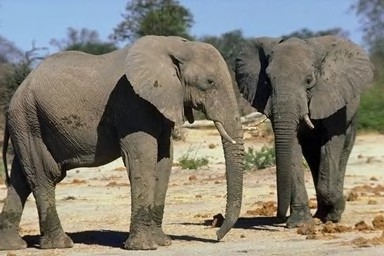
\includegraphics[width=0.5\linewidth]{\detokenize{figuras/corel_original4.jpg}}}
    \subfloat{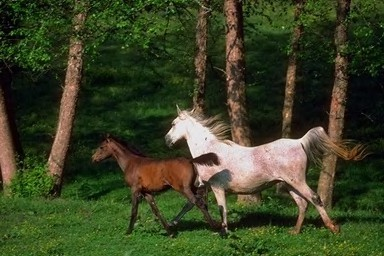
\includegraphics[width=0.5\linewidth]{\detokenize{figuras/cavalo-original2.png}}}

    \caption[Classes \emph{Cavalo} e \emph{Elefante} utilizadas neste experimento. São duas classes bem discriminadas com 100 imagens cada, originalmente da base de imagens Corel.]{Classes \emph{Cavalo} e \emph{Elefante} utilizadas neste experimento. São duas classes bem discriminadas com 100 imagens cada, originalmente da base de imagens Corel. \textit{Fonte:~Elaborado pela autora.}}
    \label{fig:resultados:1:base}
  \end{figure}
\end{minipage}

\item \textbf{Desbalanceamento}: para o sub-experimento de visualização, cada classe foi dividida em 50\% para treino e 50\% para teste, de maneira aleatória. Após, a classe \emph{Cavalo} sofreu remoção de 50\% do seu conjunto de treino, tornando-a desbalanceada. Já para a análise estatística do experimento, todas as 40 configurações de folds com $k=5$ foram realizadas (padronização anteriormente descrita na Figura~\ref{fig:folds});
\item \textbf{Método para geração artificial}: para a visualização do espaço de características foi utilizado o método de mistura de duas imagens originais, exemplificado na Figura~\ref{fig:mistura}. Para a análise do boxplot de \textit{f1-scores}, todas as gerações foram testadas;

\begin{minipage}{\linewidth}
  \begin{figure}[H]
    \subfloat[Original]{
      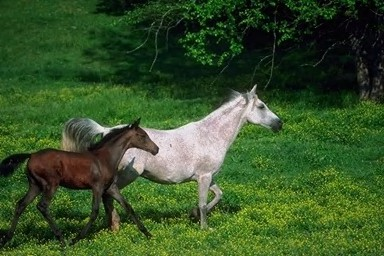
\includegraphics[width=.33\linewidth]{\detokenize{figuras/cavalo-original.png}}
    }
    \subfloat[Original]{
      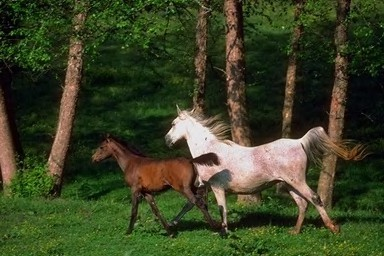
\includegraphics[width=.33\linewidth]{\detokenize{figuras/cavalo-original2.png}}
    }
    \subfloat[Mistura]{
      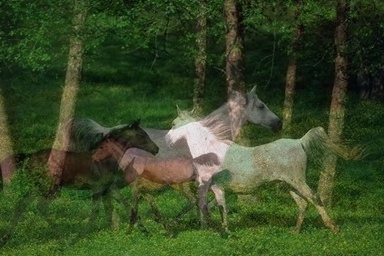
\includegraphics[width=.33\linewidth]{\detokenize{figuras/cavalo-blend.png}}
    }
    \caption[Exemplo da geração artificial de imagens com o método de mistura para as classes \emph{Elefante} e \emph{Cavalo} da Corel-1000.]{Exemplo da geração artificial de imagens com o método de mistura para as classes \emph{Elefante} e \emph{Cavalo} da Corel-1000. \textit{Fonte:~Elaborado pela autora.}}
    \label{fig:mistura}
  \end{figure}
\end{minipage}

\item \textbf{Conversão em escala de cinza}: método \emph{Intensidade} para a visualização. Todas as combinações de extração e conversão em escala de cinza foram testadas, portanto todos os métodos de conversão foram utilizados;
\item \textbf{Extração de características}: classificação de pixels de borda e interior (BIC) para a visualização. Todos os métodos de extração para a análise estatística;
\item \textbf{Classificação}: Inicialmente o classificador \textit{Naive Bayes} foi explorado, apresentando melhora na acurácia ao apenas replicar as imagens. Esse comportamento não é desejado em um classificador para a avaliação de rebalanceamento de classes. Por essa razão e por permitir uma análise da melhora no comportamento da classificação, o classificador supervisionado KNN com $K=1$ (para mais detalhes ver Seção~\ref{sec:knn}) foi utilizado;
\item \textbf{Projeção multidimensional}: dois componentes principais encontrados ao aplicar PCA (Seção~\ref{sec:pca}) nos vetores de características para redução de dimensionalidade foram projetados.
\end{enumerate}

%-------------------------------------------------------------------------------
\FloatBarrier
\item[] \textbf{Visualização}

As classes \emph{Elefante} e \emph{Cavalo} possuem 100 imagens cada. O primeiro passo foi remover imagens de uma das classes, tornando a base desbalanceada. Na Figura~\ref{fig:desbalanceado} está ilustrada a remoção de 50\% das imagens de treino da classe \emph{Cavalo}, originalmente balanceada. Essa e as próximas projeções desta seção foram obtidas com a técnica para redução de dimensionalidade PCA, descrita na Seção~\ref{sec:pca}, e são referentes aos dois componentes principais com maiores autovalores.

\begin{minipage}{\linewidth}
  \begin{figure}[H]
    \subfloat[Original]{
      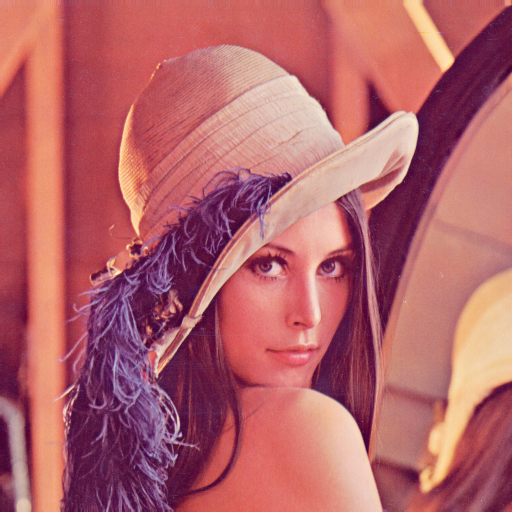
\includegraphics[width=.49\linewidth]{\detokenize{figuras/visualizacao/original.png}}
    }
    \subfloat[Desbalanceado]{
      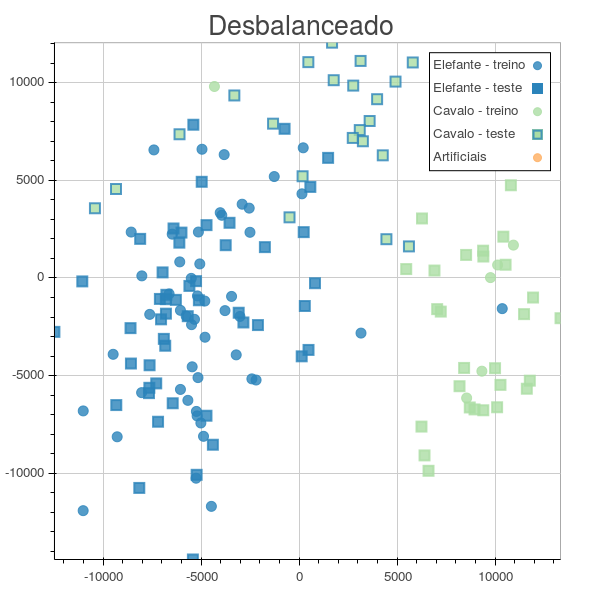
\includegraphics[width=.49\linewidth]{\detokenize{figuras/visualizacao/desbalanceado-fixed.png}}
    }
    \caption[À esquerda a projeção dos dois componentes principais obtidos com a aplicação de PCA nas classes \emph{Elefante} -- em azul -- e \emph{Cavalo} -- em verde. À direita, as mesmas classes após a remoção de 50\% das imagens de treino da classe \emph{Cavalo}. A diferença dos marcadores consiste na definição de imagens para treino e teste não existente nas classes originais.]{À esquerda a projeção dos dois componentes principais obtidos com a aplicação de PCA nas classes \emph{Elefante} -- em azul -- e \emph{Cavalo} -- em verde. À direita, as mesmas classes após a remoção de 50\% das imagens de treino da classe \emph{Cavalo}. A diferença dos marcadores consiste na definição de imagens para treino e teste não existente nas classes originais. \textit{Fonte:~Elaborado pela autora.}}
    \label{fig:desbalanceado}
  \end{figure}
\end{minipage}

Os resultados da classificação dos três experimentos (desbalanceado, SMOTE e geração artificial) utilizando KNN com $K=1$ reportou que o \textit{f1-score} da geração de imagens utilizando o método de mistura teve um ganho satisfatório em relação ao rebalanceamento no espaço de características com o SMOTE (apresentado na Figura \ref{fig:resultados:1:vis} e Tabela \ref{fig:resultados:1:tabvis}). Foi utilizado \emph{BIC} como método de extração de características e \emph{Intensidade} como método de conversão em escala de cinza. Para essa combinação, a geração de imagens utilizando mistura se mostrou favorável e portanto a visualização do espaço de características apresenta esse método como geração.

\begin{minipage}{\linewidth}
  \begin{figure}[H]
      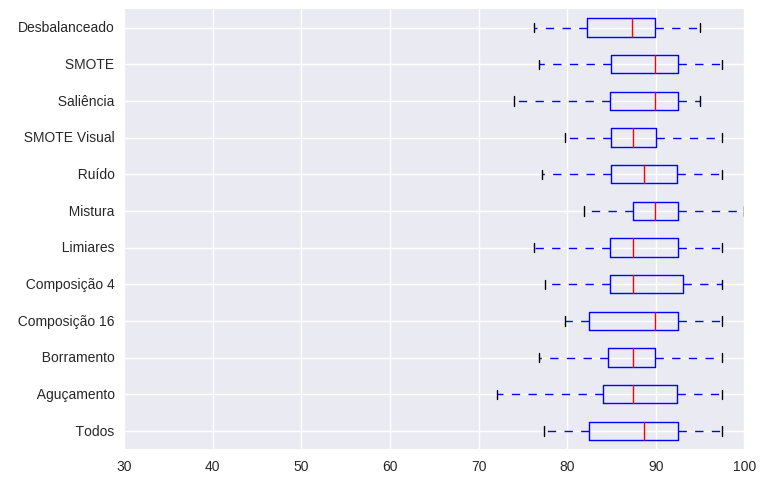
\includegraphics[width=\linewidth]{\detokenize{figuras/resultados/1/BIC_Intensity_elefante-cavalo.png}}
    \caption[Resultados de \textit{f1-score} para as classes \emph{Cavalo} e \emph{Elefante} da base Corel. Foi utilizado \emph{BIC} como método de extração de características e \emph{Intensidade} como método de conversão em escala de cinza. Para essa combinação, a geração de imagens utilizando mistura se mostrou favorável.]{Resultados de \textit{f1-score} para as classes \emph{Cavalo} e \emph{Elefante} da base Corel. Foi utilizado \emph{BIC} como método de extração de características e \emph{Intensidade} como método de conversão em escala de cinza. Para essa combinação, a geração de imagens utilizando \emph{mistura} se mostrou favorável. \textit{Fonte:~Elaborado pela autora.}}
    \label{fig:resultados:1:vis}
  \end{figure}
\end{minipage}

\meutodo{necessário a tabela reference aos f-scores da figura acima? está comentado}

% \begin{table}[!htbp]
% \centering
% \caption{Resultados de \textit{f1-score} para as classes \emph{Cavalo} e \emph{Elefante}, utilizando \emph{Intensidade} como método para conversão em escala de cinza e \emph{BIC} para extração de características.}
% \label{fig:resultados:1:tabvis}
% \begin{tabular}{|l|c|c|}
% \hline
% \textbf{Intensidade e BIC} & \textbf{Média} & \textbf{Desvio padrão} \\ \hline
% Todos                      & 88.07          & 5.30                   \\ \hline
% Aguçamento                 & 86.65          & 7.00                   \\ \hline
% Borramento                 & 87.17          & 5.10                   \\ \hline
% Composição 16              & 88.16          & 5.32                   \\ \hline
% Composição 4               & 88.12          & 5.45                   \\ \hline
% Limiares                   & 87.65          & 5.10                   \\ \hline
% Mistura                    & \textbf{88.84} & 5.03          \\ \hline
% Ruído                      & 87.95          & 5.75                   \\ \hline
% SMOTE Visual               & 87.69          & 5.28                   \\ \hline
% Saliência                  & 88.09          & 5.58                   \\ \hline
% SMOTE                      & 88.55          & 5.21                   \\ \hline
% Desbalanceado              & 85.82          & 5.69                   \\ \hline
% \end{tabular}
% \end{table}

Para verificar se a geração de imagens inseriu mais informação na classe minoritária do que apenas povoar os espaços entre os exemplos (i.e.\ SMOTE), a classe rebalanceada utilizando ambos métodos está demonstrada na Figura~\ref{fig:compara_vis_treino_fixed}. Em laranja estão representados os novos exemplos de treinamento, projetados no plano da base original balanceada.

\begin{minipage}{\linewidth}
  \begin{center}
  \begin{figure}[H]
    \subfloat[Smote]{      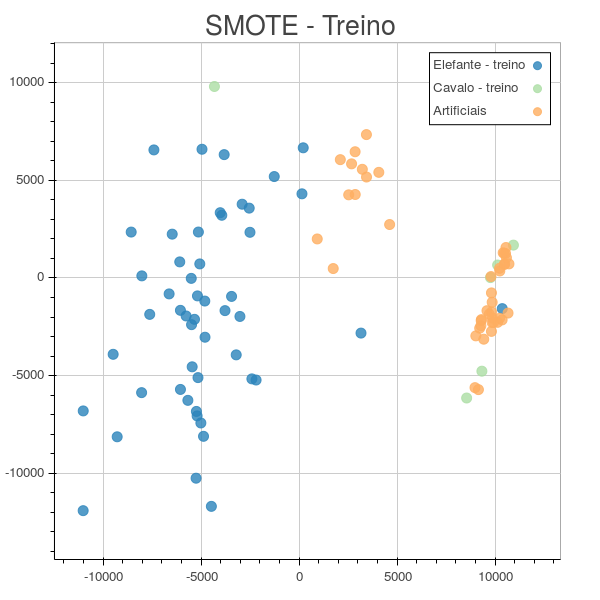
\includegraphics[width=.5\linewidth]{\detokenize{figuras/visualizacao/smote-treino-fixed.png}}
    }
    \subfloat[Geração artificial]{      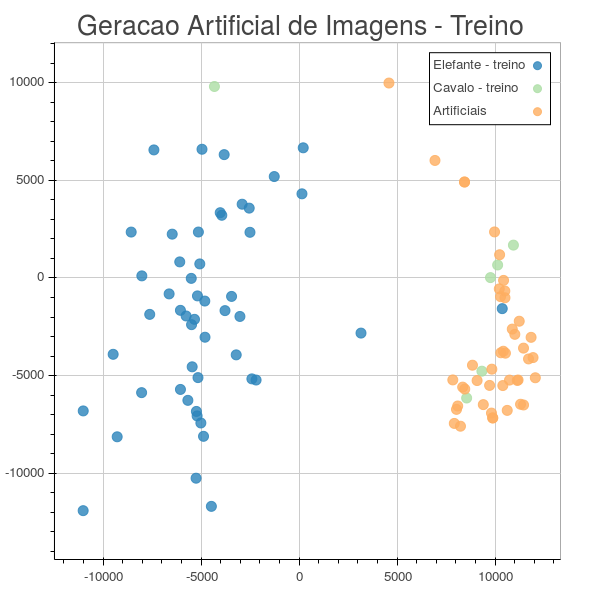
\includegraphics[width=.5\linewidth]{\detokenize{figuras/visualizacao/geracao-treino-fixed.png}}
    }
  \caption[Comparação dos exemplos de treinamento da geração com SMOTE e no campo visual. Em laranja estão representados os novos exemplos, projetados no plano da base original balanceada.]{Comparação dos exemplos de treinamento da geração com SMOTE e no campo visual. Em laranja estão representados os novos exemplos, projetados no plano da base original balanceada. \textit{Fonte:~Elaborado pela autora.}}
  \label{fig:compara_vis_treino_fixed}
  \end{figure}
  \end{center}
\end{minipage}

Após o treinamento realizado com as novas imagens geradas e as originais, o conjunto de teste foi fornecido ao classificador 1-NN e o resultado das predições está ilustrado na Figura~\ref{fig:compara_vis_teste}. A cor no interior dos marcadores quadrados representa a classe real dos exemplos e a borda representa a classe predita pelo classificador. Nota-se que a melhoria na classificação com a geração de imagens fica visível e corresponde ao aumento do \textit{f1-score}.


\begin{minipage}{\linewidth}
  \begin{figure}[H]
    \subfloat[Smote]{
      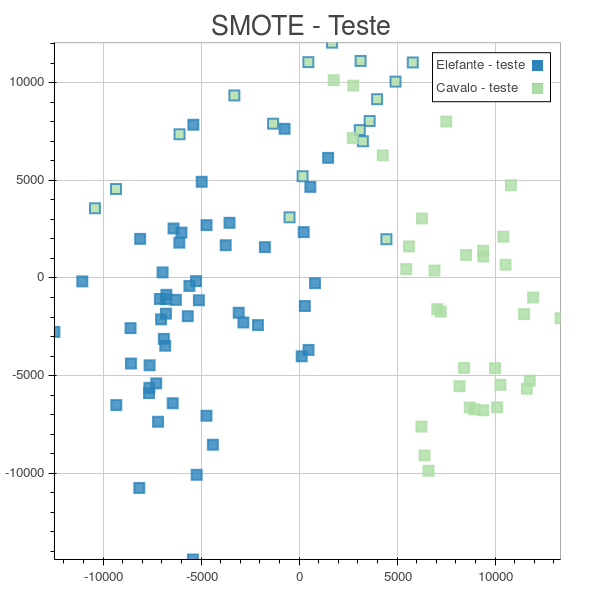
\includegraphics[width=.5\linewidth]{\detokenize{figuras/visualizacao/smote-teste-fixed.png}}
    }
    \subfloat[Geração artificial]{
      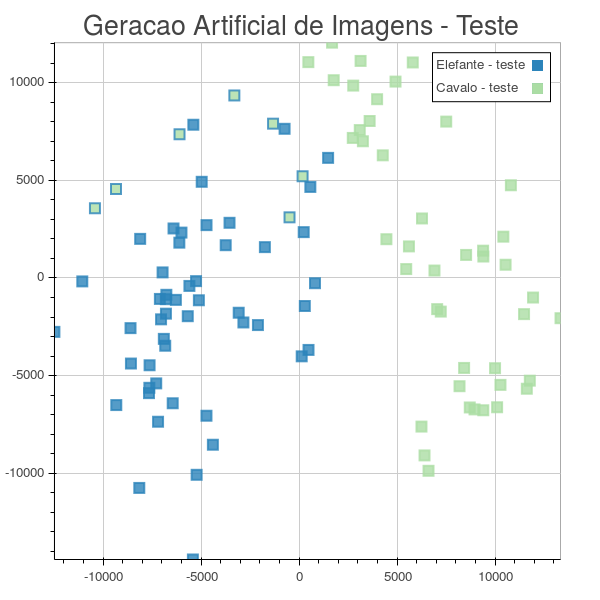
\includegraphics[width=.5\linewidth]{\detokenize{figuras/visualizacao/geracao-teste-fixed.png}}
    }
  \caption[Resultado do teste da classificação com 1-NN após o treinamento realizado com as bases rebalanceadas. A cor no interior dos marcadores quadrados representa a classe real dos exemplos e a borda representa a classe predita pelo classificador.]{Resultado do teste da classificação com 1-NN após o treinamento realizado com as bases rebalanceadas. A cor no interior dos marcadores quadrados representa a classe real dos exemplos e a borda representa a classe predita pelo classificador. \textit{Fonte:~Elaborado pela autora.}}
  \label{fig:compara_vis_teste}
\end{figure}
\end{minipage}

De uma forma geral, pode-se dizer que a geração de imagens melhorou a definição da classe minoritária e foi o método que mais se assemelhou à distribuição dos dados originais. Além disso, um dos problemas do SMOTE pode ser verificado nessas projeções: \textbf{ao realizar a interpolação dos vetores de características originais, exemplos podem ser criados em regiões do espaço que fazem parte da outra classe}. Ficou claro também que o método SMOTE não possui capacidade de extrapolar a sua região, como pode ser observado no grupo de exemplos gerados à direita do espaço de características. O SMOTE gerou novos elementos próximos a uma linha reta, enquanto a geração de imagens proporcionou uma abrangência maior em volta desse espaço, com maior dispersão.

Na Figura \ref{fig:region} é possível visualizar a região de decisão, observando suas modificações frente aos métodos. Pode ser observado que em ambas técnicas a região da classe minoritária apresenta-se melhor representada. Além disso, é possível verificar que o SMOTE ocasionou uma certa ``invasão'' do espaço de características da classe majoritária.

\begin{minipage}{\linewidth}
  \begin{figure}[H]
    \begin{center}
    \subfloat[Desbalanceado]{
      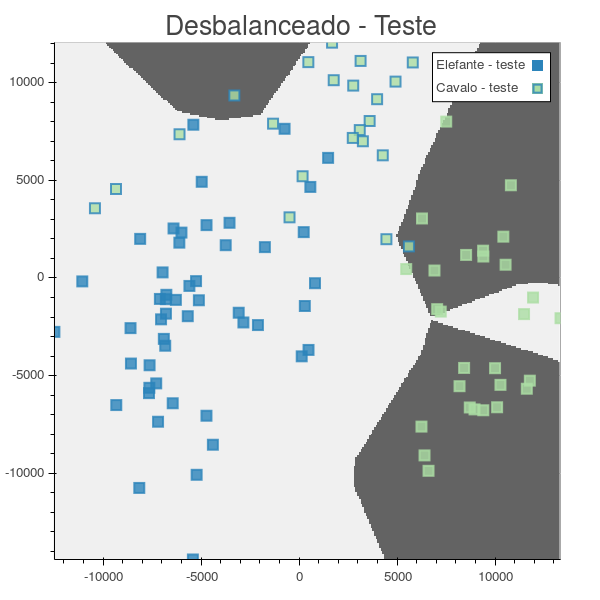
\includegraphics[width=.5\linewidth]{\detokenize{figuras/visualizacao/desbalanceado-teste-region.png}}
    }
    \end{center}
    \subfloat[Smote]{
      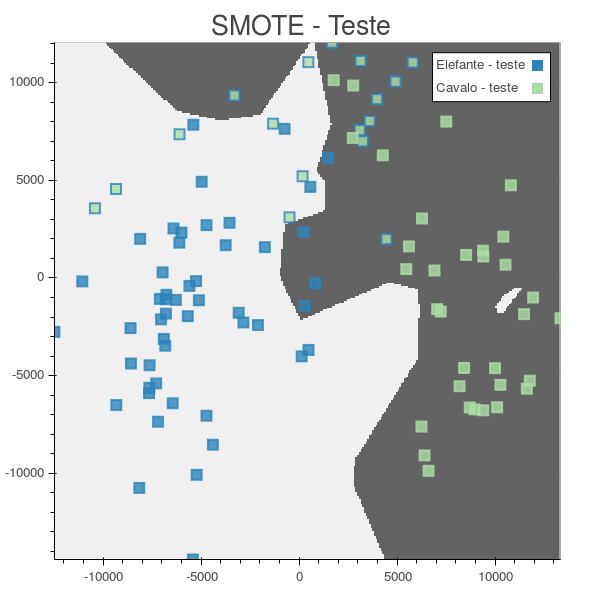
\includegraphics[width=.5\linewidth]{\detokenize{figuras/visualizacao/smote-teste-region.png}}
    }
    \subfloat[Geração artificial]{
      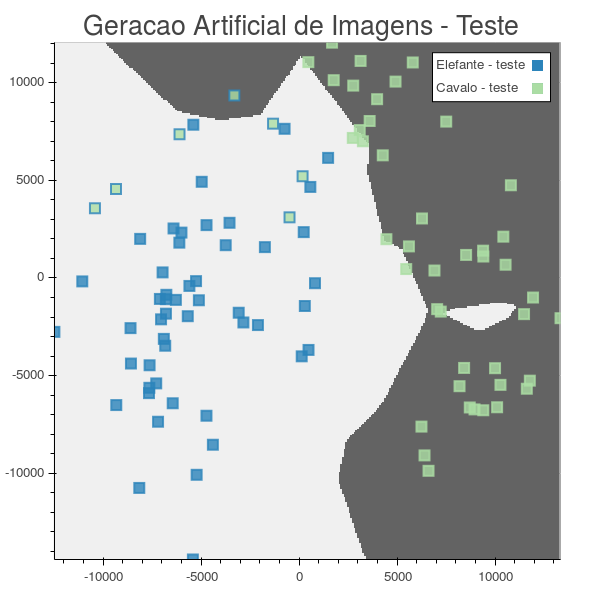
\includegraphics[width=.5\linewidth]{\detokenize{figuras/visualizacao/geracao-teste-region.png}}
    }
  \caption[Região de decisão com K-NN (K = 1). Pode ser observado que em ambas técnicas a região da classe minoritária apresenta-se melhor representada. Além disso, é possível verificar que o SMOTE ocasionou uma certa ``invasão'' do espaço de características da classe majoritária.]{Região de decisão com K-NN (K = 1). Pode ser observado que em ambas técnicas a região da classe minoritária apresenta-se melhor representada. Além disso, é possível verificar que o SMOTE ocasionou uma certa ``invasão'' do espaço de características da classe majoritária. \textit{Fonte:~Elaborado pela autora.}}
  \label{fig:region}
  \end{figure}
\end{minipage}

Em todas as figuras anteriores relacionadas a essa visualização, os exemplos foram projetados no plano criado pelas suas componentes principais com maior autovalores da base original balanceada. Se após a geração de novos exemplos essas componentes forem recalculadas (Figura \ref{fig:compara_vis_treino}), pode-se notar que a geração de imagens artificiais proporciona a criação de um subespaço que melhor discretiza as classes, quando comparado com SMOTE ou com a base desbalanceada.

\begin{minipage}{\linewidth}
  \begin{figure}[H]
    \begin{center}
    \subfloat[Desbalanceado]{
      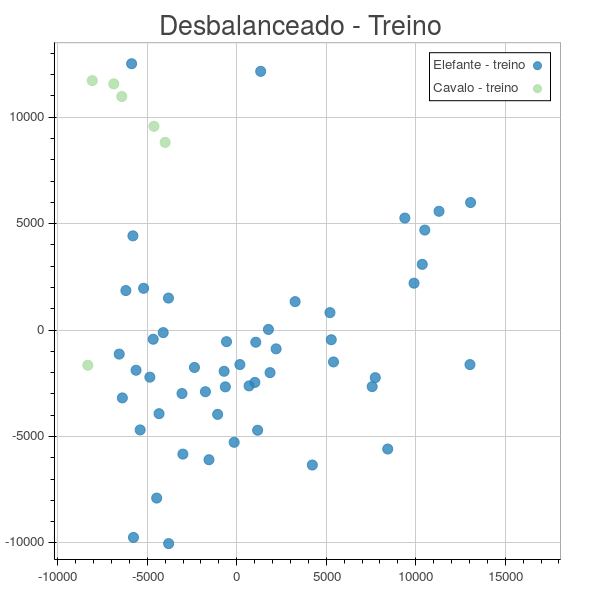
\includegraphics[width=.5\linewidth]{\detokenize{figuras/visualizacao/desbalanceado-treino.png}}
    }
    \end{center}
    \subfloat[Smote]{
      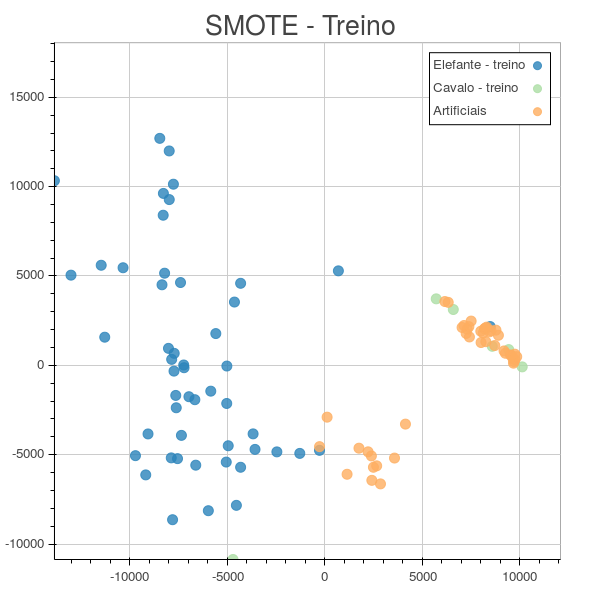
\includegraphics[width=.5\linewidth]{\detokenize{figuras/visualizacao/smote-treino.png}}
    }
    \subfloat[Geração artificial]{
      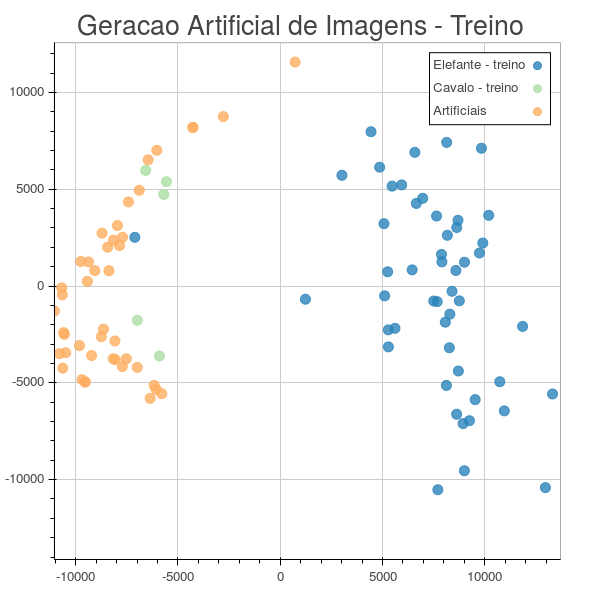
\includegraphics[width=.5\linewidth]{\detokenize{figuras/visualizacao/geracao-treino.png}}
    }
  \caption[Melhores subespaços encontrados após a geração de novos exemplos para o SMOTE e para a geração artificial de imagens, e após a remoção de imagens para a projeção dos dados desbalanceados. Pode-se notar que a geração de imagens artificiais proporciona a criação de um subespaço que melhor discretiza as classes, quando comparado com SMOTE ou com a base desbalanceada.]{Melhores subespaços encontrados após a geração de novos exemplos para o SMOTE e para a geração artificial de imagens, e após a remoção de imagens para a projeção dos dados desbalanceados. Pode-se notar que a geração de imagens artificiais proporciona a criação de um subespaço que melhor discretiza as classes, quando comparado com SMOTE ou com a base desbalanceada. \textit{Fonte:~Elaborado pela autora.}}
  \label{fig:compara_vis_treino}
  \end{figure}
\end{minipage}

Como relatado no início desse experimento, o extrator de características utilizado foi o \emph{BIC}. Fundamentalmente ele captura informações de intensidade de cor das imagens. Na Figura~\ref{fig:vis_images} as próprias imagens foram utilizadas como marcadores na projeção do melhor subespaço após a geração artificial com o método de \emph{mistura}. É nítido o impacto da etapa de extração de características na separação das classes e também no método de geração de imagens antes de tal extração.

\begin{minipage}{\linewidth}
  \begin{figure}[H]
    \begin{center}
      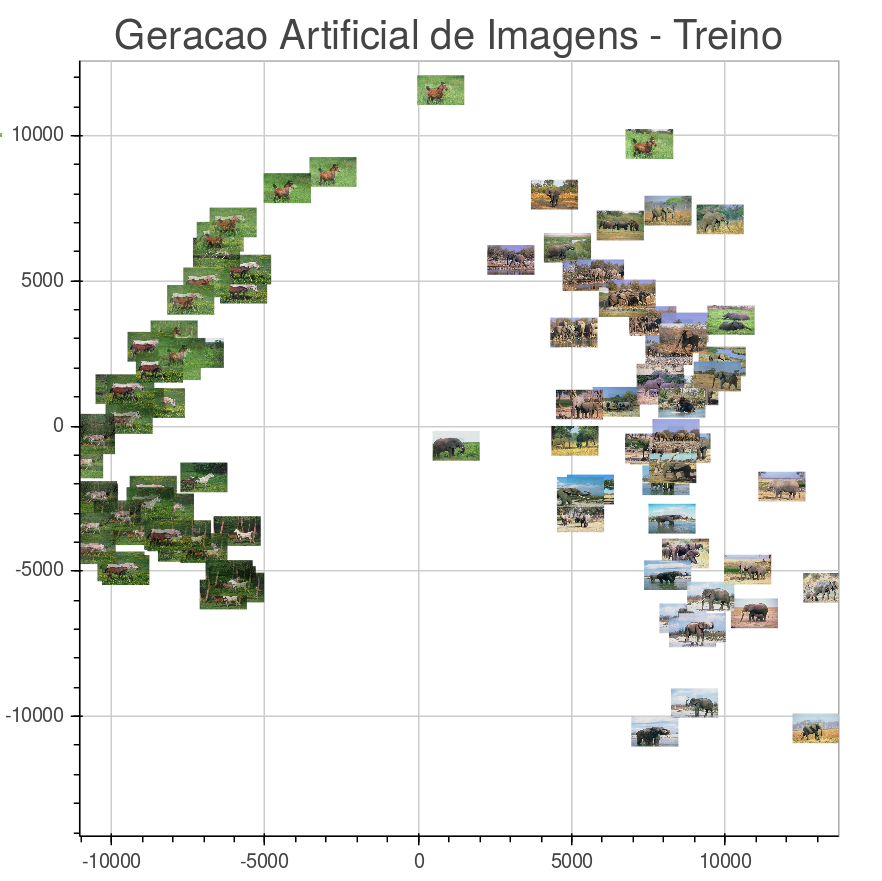
\includegraphics[width=.7\linewidth]{\detokenize{figuras/visualizacao/vis-images.png}}
    \end{center}
  \caption[Visualização do impacto do método de extração de características na separação entre classes. Possível verificar que o BIC utiliza as intensidades como principal representação de uma imagem.]{Visualização do impacto do método de extração de características na separação entre classes. Possível verificar que o BIC utiliza as intensidades como principal representação de uma imagem. \textit{Fonte:~Elaborado pela autora.}}
  \label{fig:vis_images}
\end{figure}
\end{minipage}

%-------------------------------------------------------------------------------
\item[] \textbf{Resultados: melhor combinação dos métodos de extração de características e conversão para escala de cinza}

Para análise estatística, todas as combinações de conversão para escala de cinza e métodos de extração de características foram utilizados. A combinação que obteve o melhor \textit{f-score} para as classes \emph{Elevante} e \emph{Cavalo} foi utilizando \emph{Gleam} e \emph{ACC}. O \textit{boxplot} apresentado na Figura \ref{fig:resultados:1:melhor} retrata a média dos \textit{f-scores} das 40 configurações deste experimento. O método \emph{mistura}, exemplificado na Figura \ref{fig:resultados:1:mistura}, obteve o melhor \textit{f-score}. A Tabela \ref{fig:resultados:1:tabmelhor} mostra os valores de tal métrica com valores decimais para o cálculo dos testes estatísticos.

\begin{minipage}{\linewidth}
  \begin{figure}[H]
  \begin{center}
      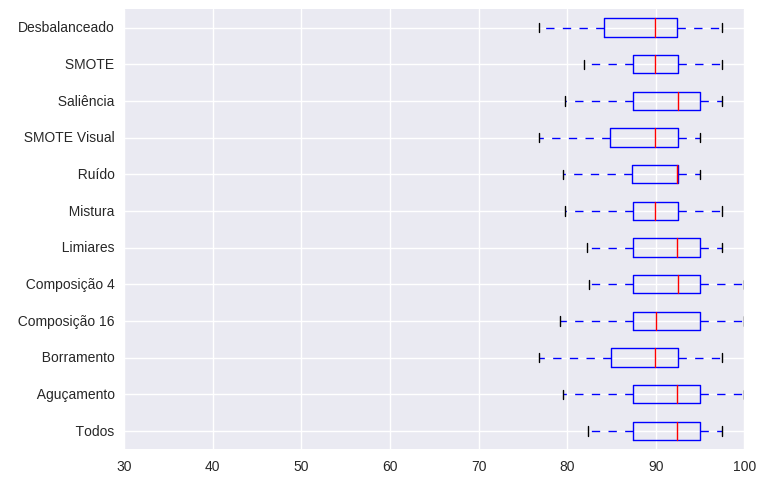
\includegraphics[width=\linewidth]{\detokenize{figuras/resultados/1/ACC_Gleam_elefante-cavalo.png}}
  \end{center}
  \caption[]{Conversão em escala de cinza com Gleam e ACC como método de extração de características. \textit{Fonte:~Elaborado pela autora.}}
  \label{fig:resultados:1:melhor}
\end{figure}
\end{minipage}

\begin{minipage}{\linewidth}
  \begin{figure}[H]
    \subfloat[Original]{
      \includegraphics[width=.33\linewidth]{\detokenize{figuras/resultados/1/original-mistura.png}}
    }
    \subfloat[Original]{
      \includegraphics[width=.33\linewidth]{\detokenize{figuras/resultados/1/original2-mistura.png}}
      }
    \subfloat[Mistura]{
      \includegraphics[width=.33\linewidth]{\detokenize{figuras/resultados/1/resultado-mistura.png}}
    }
   \caption[]{ \textit{Fonte:~Elaborado pela autora.}}
   \label{fig:resultados:1:mistura}
  \end{figure}
\end{minipage}

\begin{table}[!htbp]
\centering
\caption{Resultados de \textit{f1-score} para as classes \emph{Cavalo} e \emph{Elefante}, utilizando \emph{Gleam} como método para conversão em escala de cinza e \emph{ACC} para extração de características.}
\label{fig:resultados:1:tabmelhor}
\begin{tabular}{|l|c|c|}
\hline
\textbf{Gleam \& ACC} & \textbf{Média}     & \textbf{Desvio Padrão} \\ \hline
Todos                 & 91.090913          & 4.559066               \\ \hline
Aguçamento            & 91.002678          & 4.907016               \\ \hline
Borramento            & 89.394500          & 5.103498               \\ \hline
Composição 16         & 90.934305          & 4.399334               \\ \hline
Composição 4          & \textbf{91.773528} & 4.909852               \\ \hline
Limiares              & 90.893133          & 5.285833               \\ \hline
Mistura               & 90.177055          & 4.409787               \\ \hline
Ruído                 & 89.337770          & 5.169757               \\ \hline
SMOTE Visual          & 88.616535          & 5.567976               \\ \hline
Saliência             & 91.282655          & 4.230281               \\ \hline
SMOTE                 & 90.169505          & 4.498590               \\ \hline
Desbalanceado         & 88.258567          & 5.538461               \\ \hline
\end{tabular}
\end{table}

%-------------------------------------------------------------------------------
\item[] \textbf{Resultados: maior variância obtida com a combinação dos métodos de extração de características e conversão para escala de cinza}

Considerando a análise da melhor combinação dos métodos de representação da imagem, foi verificado também a performance dos rebalanceamentos em um cenário mais complicado: o de maior variância dos \textit{f-scores} para as 40 configurações da validação. A Figura \ref{fig:resultados:1:pior} mostra o \textit{boxplot} referente aos resultados da Tabela \ref{fig:resultados:1:tabpior}. O melhor método de rebalanceamento para tal cenário foi de geração artificial de imagens aplicando \emph{ruído} nas imagens originais e as utilizando como treinamento (exemplificado na Figura \ref{fig:resultados:1:ruido}).

\begin{minipage}{\linewidth}
  \begin{figure}[H]
    \begin{center}
      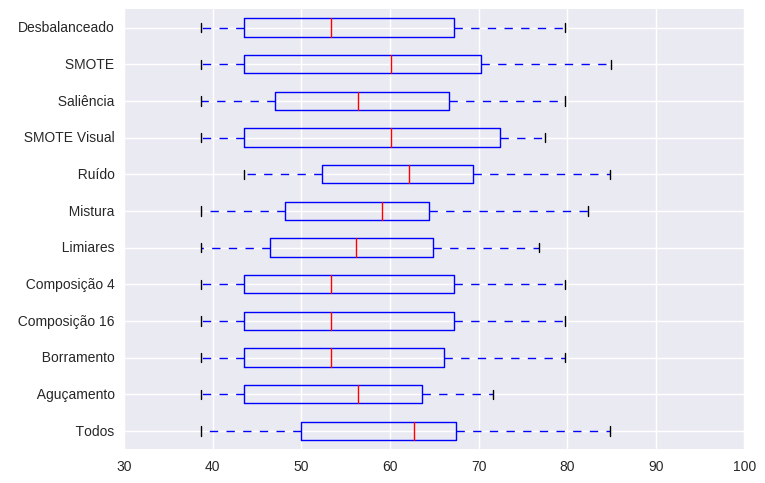
\includegraphics[width=\linewidth]{\detokenize{figuras/resultados/1/HOG_MSB_elefante-cavalo.png}}
    \end{center}
    \caption[Conversão em escala de cinza com MSB e HOG como método de extração de características. ]{Conversão em escala de cinza com MSB e HOG como método de extração de características. \textit{Fonte:~Elaborado pela autora.}}
    \label{fig:resultados:1:pior}
  \end{figure}
\end{minipage}

\begin{table}[!htbp]
\centering
\caption{Resultados de \textit{f1-score} para as classes \emph{Cavalo} e \emph{Elefante}, utilizando \emph{MSB} como método para conversão em escala de cinza e \emph{HOG} para extração de características.}
\label{fig:resultados:1:tabpior}
\begin{tabular}{|l|c|c|}
\hline
\textbf{MSB \& HOG} & \textbf{Média}     & \textbf{Desvio Padrão} \\ \hline
Todos               & 60.000127          & 12.063967              \\ \hline
Aguçamento          & 54.809555          & 10.610213              \\ \hline
Borramento          & 55.588173          & 13.275734              \\ \hline
Composição 16       & 55.667145          & 13.341421              \\ \hline
Composição 4        & 55.652205          & 13.323408              \\ \hline
Limiares            & 55.652268          & 11.547820              \\ \hline
Mistura             & 57.826535          & 10.882912              \\ \hline
Ruído               & \textbf{62.174910} & 10.746760              \\ \hline
SMOTE Visual        & 58.920085          & 14.765860              \\ \hline
Saliência           & 56.322367          & 12.169296              \\ \hline
SMOTE               & 58.342450          & 13.768688              \\ \hline
Desbalanceado       & 55.667145          & 13.341421              \\ \hline
\end{tabular}
\end{table}

\begin{minipage}{\linewidth}
  \begin{figure}[H]
    \subfloat[Original]{
      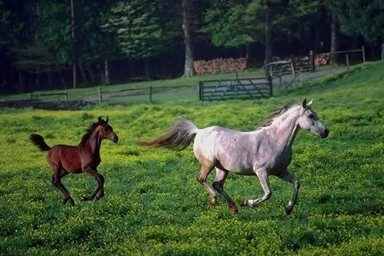
\includegraphics[width=.5\linewidth]{\detokenize{figuras/resultados/1/original-ruido.png}}
    }
    \subfloat[Ruído]{
      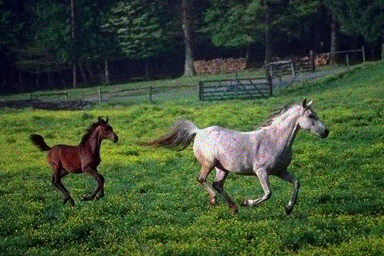
\includegraphics[width=.5\linewidth]{\detokenize{figuras/resultados/1/resultado-ruido.png}}
    }
 \caption[]{ \textit{Fonte:~Elaborado pela autora.}}
 \label{fig:resultados:1:ruido}
\end{figure}
\end{minipage}

%-------------------------------------------------------------------------------
\item[] \textbf{Discussão}
\meutodo{Adicionar um item de discussão, para recapitular tudo aqui? talvez fique repetitivo}

\end{itemize}

%%%%%%%%%%%%%%%%%%%%%%%%%%%%%%%%%%%%%%%%%%%%%%%%%%%%%%%%%%%%%%%%%%%%%%%%%%%%%%%%
\FloatBarrier
\subsection{Experimento 2: duas classes bem sobrepostas}

O experimento anterior considerou classes distintas, por isso classes de difícil diferenciação também foram testadas.

\begin{itemize}
%-------------------------------------------------------------------------------
\item[] \textbf{Protocolo}
\begin{enumerate}
\item \textbf{Classes de imagens originais}: as classes \textit{Praia} e \emph{Montanha} foram escolhidas por serem as classes que possuem maior dificuldade de diferenciação da base Corel, havendo alta taxa de sobreposição de intensidades de cores e texturas, conforme testes realizados.

\item \textbf{Desbalanceamento}: as duas classes contém 100 imagens cada, portanto são balanceadas. Para o experimento, foram utilizadas as 40 configurações de $k=5$ folds.

\item \textbf{Método para geração artificial}: todas as gerações foram testadas, as que melhor se sobressaíram são relatadas nas seções de resultados a seguir.

\item \textbf{Quantização}: todos os métodos de conversão em escala de cinza foram testados.

\item \textbf{Extração de características}: todos os métodos para extração foram testados.

\item \textbf{Classificação}: o classificador utilizado foi o KNN com $K=1$.
\end{enumerate}

%-------------------------------------------------------------------------------
\item[] \textbf{Resultados: melhor combinação dos métodos de extração e conversão para escala de cinza}

A combinação de métodos que resultou em um melhor \textit{f-score} para esse contexto foi a utilização de Luminância e BIC. Na Figura \ref{fig:resultados:2:melhor} é possível verificar o \textit{boxplot} dos \textit{f-scores} para as classes desbalanceadas, rebalanceadas com SMOTE após a extração de características e rebalanceadas com os métodos de geração artificial como primeiro passo do \textit{pipeline}. Como pode ser visto na Tabela \ref{tab:resultados:2:melhor}, diversos métodos foram melhores que o SMOTE, e todos melhores do que a base desbalanceada. O método de saliência, mistura e composição obtiveram os melhores resultados.

\begin{figure}[!htbp]
  \begin{center}
      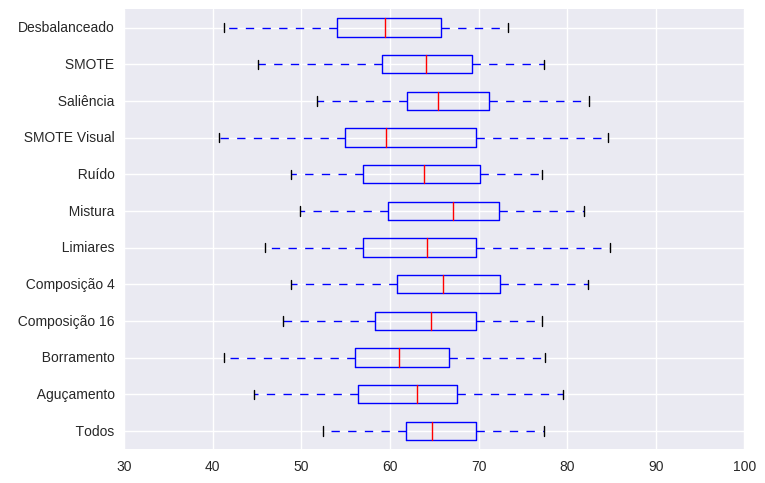
\includegraphics[width=\linewidth]{\detokenize{figuras/resultados/2/BIC_Luminance_praia-montanha.png}}
  \end{center}
  \caption[Boxplot das classes \emph{Praia} e \emph{Montanha} para a conversão em escala de cinza com Luminância e BIC como método de extração de características.]{Boxplot das classes \emph{Praia} e \emph{Montanha} para a conversão em escala de cinza com Luminância e BIC como método de extração de características. \textit{Fonte:~Elaborado pela autora.}}
  \label{fig:resultados:2:melhor}
\end{figure}

\begin{table}[!htbp]
\centering
\caption{Resultados de \textit{f1-score} para as classes \emph{Praia} e \emph{Montanha}, utilizando \emph{Luminância} como método para conversão em escala de cinza e \emph{BIC} para extração de características.}
\label{tab:resultados:2:melhor}
\begin{tabular}{|l|c|c|}
\hline
\textbf{Luminância e BIC} & \textbf{Média} & \textbf{Desvio padrão} \\ \hline
Todos                  & 65.21          & 7.54                   \\ \hline
Aguçamento             & 62.30          & 7.85                   \\ \hline
Borramento             & 61.24          & 7.55                   \\ \hline
Composição 16          & 64.23          & 7.31                   \\ \hline
Composição 4           & 65.65          & 8.27                   \\ \hline
Limiares               & 63.69          & 8.77                   \\ \hline
Mistura                & 65.41          & 8.20                   \\ \hline
Ruído                  & 63.50          & 8.05                   \\ \hline
SMOTE Visual           & 61.55          & 9.44                   \\ \hline
Saliência              & \textbf{65.69} & 6.63                   \\ \hline
SMOTE                  & 63.58          & 7.74                   \\ \hline
Desbalanceado          & 59.49          & 8.11                   \\ \hline
\end{tabular}
\end{table}

A Figura \ref{fig:resultados:2:saliencia} exemplifica uma geração artificial deste experimento, utilizando o método de \emph{saliência}. Interessante notar que essa imagem faz sentido visualmente.

\begin{minipage}{\linewidth}
  \begin{figure}[H]
    \subfloat[Original]{  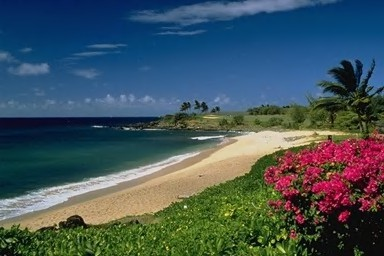
\includegraphics[width=.33\linewidth]{\detokenize{figuras/resultados/2/original-saliencia.png}}
    }
    \subfloat[Original]{
      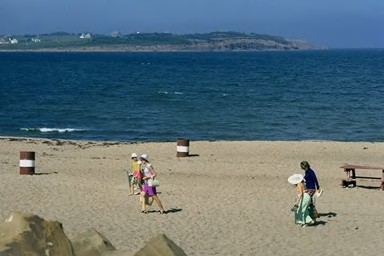
\includegraphics[width=.33\linewidth]{\detokenize{figuras/resultados/2/original2-saliencia.png}}
    }
    \subfloat[Saliência]{
      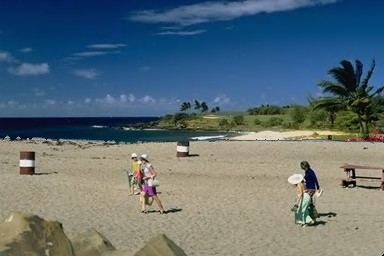
\includegraphics[width=.33\linewidth]{\detokenize{figuras/resultados/2/resultado-saliencia.png}}
    }
 \caption[Geração artificial utilizando o método de \emph{saliência} em duas imagens da classe \emph{Praia} da base de imagens Corel.]{Geração artificial utilizando o método de \emph{saliência} em duas imagens da classe \emph{Praia} da base de imagens Corel. \textit{Fonte:~Elaborado pela autora.}}
 \label{fig:resultados:2:saliencia}
\end{figure}
\end{minipage}

%-------------------------------------------------------------------------------
\item[] \textbf{Resultados: maior variância obtida com a combinação dos métodos de extração e conversão para escala de cinza}

Os métodos que combinados obtiveram a maior variância foram \emph{Intensidade} e \emph{HOG} (ver Figura \ref{fig:resultados:2:pior} e Tabela \ref{tab:resultados:2:pior}). O rebalanceamento com a geração de imagens obteve a melhor performance. Porém, o único método que melhorou a variância foi o \emph{aguçamento} (um exemplo de tal geração pode ser visto na Figura \ref{fig:resultados:2:agucamento}). A Figura \ref{fig:resultados:2:mistura} exemplifica a geração artificial com o método \emph{mistura}, utilizando duas imagens de treinamento da classe \emph{Montanha}.

\begin{minipage}{\linewidth}
  \begin{figure}[H]
  \begin{center}
      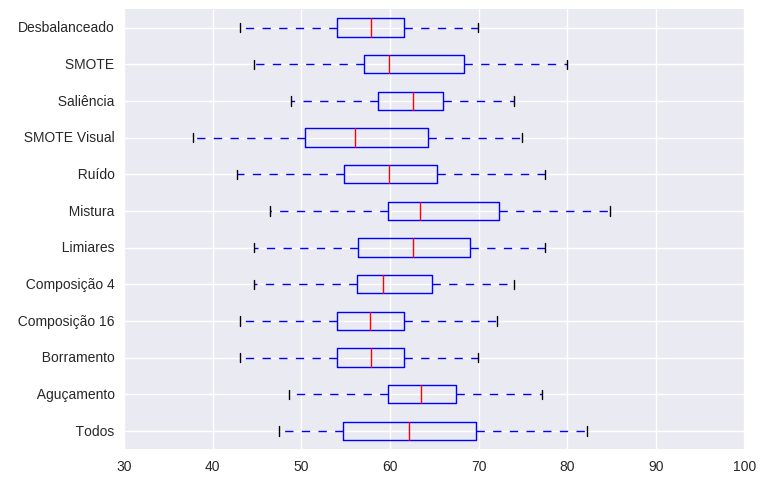
\includegraphics[width=\linewidth]{\detokenize{figuras/resultados/2/HOG_Intensity_praia-montanha.png}}
  \end{center}
  \caption[]{Conversão em escala de cinza com Intensidade e HOG como método de extração de características. \textit{Fonte:~Elaborado pela autora.}}
  \label{fig:resultados:2:pior}
\end{figure}
\end{minipage}

\begin{table}[!htbp]
\centering
\caption{Resultados de \textit{f1-score} para as classes \emph{Praia} e \emph{Montanha}, utilizando \emph{Intensidade} como método para conversão em escala de cinza e \emph{HOG} para extração de características.}
\label{tab:resultados:2:pior}
\begin{tabular}{|l|c|c|}
\hline
\textbf{Intensidade e HOG} & \textbf{Média}     & \textbf{Desvio padrão} \\ \hline
Todos                      & 62.184222          & 9.310391               \\ \hline
Aguçamento                 & 63.455343          & 6.719545               \\ \hline
Borramento                 & 57.599052          & 8.332506               \\ \hline
Composição 16              & 57.669325          & 8.424716               \\ \hline
Composição 4               & 59.239965          & 8.254027               \\ \hline
Limiares                   & 63.138800          & 9.132368               \\ \hline
Mistura                    & \textbf{65.255990} & 9.073246               \\ \hline
Ruído                      & 60.577283          & 8.690926               \\ \hline
SMOTE Visual               & 56.998855          & 9.050991               \\ \hline
Saliência                  & 61.728330          & 8.154174               \\ \hline
SMOTE                      & 62.210017          & 8.318301               \\ \hline
Desbalanceado              & 57.651543          & 8.323832               \\ \hline
\end{tabular}
\end{table}

% \begin{minipage}{\linewidth}
%   \begin{figure}[H]
%     \subfloat[Original]{
%       \includegraphics[width=.33\linewidth]{\detokenize{figuras/resultados/2/original-agucamento.png}}
%     }
%     \subfloat[Original]{
%       \includegraphics[width=.33\linewidth]{\detokenize{figuras/resultados/2/original2-agucamento.png}}
%     }
%     \subfloat[Mistura]{
%       \includegraphics[width=.33\linewidth]{\detokenize{figuras/resultados/2/resultado-agucamento.png}}
%     }
%     \caption[Geração artificial utilizando o método de \emph{aguçamento} em duas imagens da classe \emph{Montanha} da base de imagens Corel.]{Geração artificial utilizando o método de \emph{aguçamento} em duas imagens da classe \emph{Montanha} da base de imagens Corel. \textit{Fonte:~Elaborado pela autora.}}
%     \label{fig:resultados:2:agucamento}
%   \end{figure}
% \end{minipage}


\begin{minipage}{\linewidth}
  \begin{figure}[H]
    \subfloat[Original]{
      \includegraphics[width=.33\linewidth]{\detokenize{figuras/resultados/2/original-mistura.png}}
    }
    \subfloat[Original]{
      \includegraphics[width=.33\linewidth]{\detokenize{figuras/resultados/2/original2-mistura.png}}
    }
    \subfloat[Mistura]{
      \includegraphics[width=.33\linewidth]{\detokenize{figuras/resultados/2/resultado-mistura.png}}
    }
    \caption[Geração artificial utilizando o método de \emph{mistura} em duas imagens da classe \emph{Montanha} da base de imagens Corel.]{Geração artificial utilizando o método de \emph{mistura} em duas imagens da classe \emph{Montanha} da base de imagens Corel. \textit{Fonte:~Elaborado pela autora.}}
    \label{fig:resultados:2:mistura}
  \end{figure}
\end{minipage}

%-------------------------------------------------------------------------------
\item[] \textbf{Discussão}

\end{itemize}

%%%%%%%%%%%%%%%%%%%%%%%%%%%%%%%%%%%%%%%%%%%%%%%%%%%%%%%%%%%%%%%%%%%%%%%%%%%%%%%%
\FloatBarrier
\subsection{Experimento 3: multiclasses}

Os dois experimentos anteriores analisaram o rebalanceamento de apenas duas classes. Este experimento apresenta a geração artificial de imagens aplicada a uma base com 10 classes balanceadas, contendo 100 imagens cada.

\begin{itemize}
%-------------------------------------------------------------------------------
\item[] \textbf{Protocolo}

O seguinte protocolo foi seguido para a obtenção dos resultados:

\begin{enumerate}
\item \textbf{Classes de imagens originais}: esse experimento foi realizado com a base de imagens Corel-1000\footnote{Disponível em http://wang.ist.psu.edu/docs/related/}, composta por fotografias que representam classes variadas: tribos africanas, praia, construções, ônibus, dinossauros, elefantes, flores, cavalos, montanhas e tipos de comidas.. Para fins de exemplificação, são apresentadas amostras das imagens que representam essas classes na Figura \ref{fig:resultados:3:base}.

\begin{minipage}{\linewidth}
  \begin{figure}[H]
    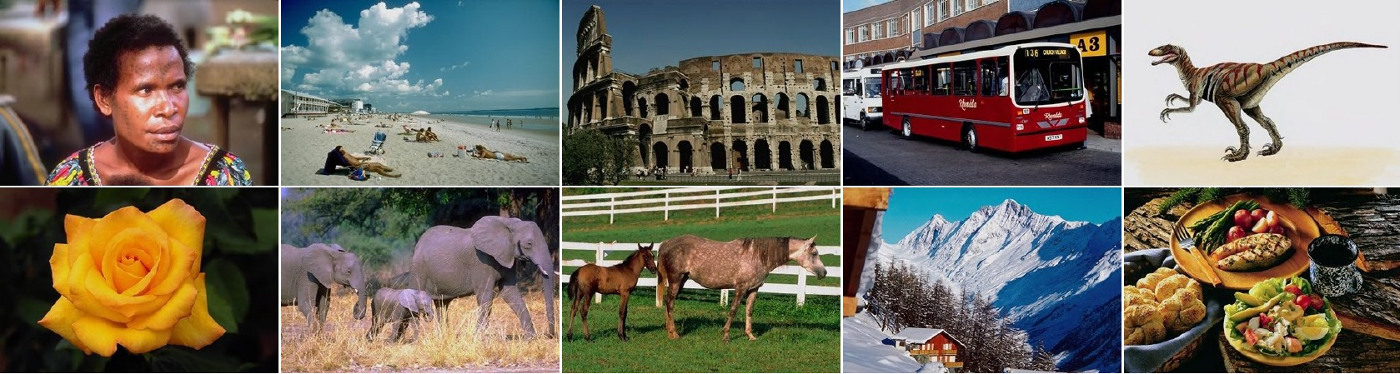
\includegraphics[width=\linewidth]{\detokenize{figuras/quantizacao/fig_COREL_dataset.jpg}}
    \caption{Base de imagens Corel-1000. \textit{Fonte:~\cite{Ponti2016}.}}
    \label{fig:resultados:3:base}
  \end{figure}
\end{minipage}

\item \textbf{Desbalanceamento}: 200 configurações de folds para que cada classe fosse desbalanceada.
\item \textbf{Método para geração artificial}: o melhor foi a mistura.

\begin{minipage}{\linewidth}
  \begin{figure}[H]
    \subfloat[Original]{
      \includegraphics[width=.33\linewidth]{\detokenize{figuras/resultados/3/original-mistura.png}}
    }
    \subfloat[Original]{
      \includegraphics[width=.33\linewidth]{\detokenize{figuras/resultados/3/original2-mistura.png}}
    }
    \subfloat[Mistura]{
      \includegraphics[width=.33\linewidth]{\detokenize{figuras/resultados/3/resultado-mistura.png}}
    }
    \caption{}
    \label{fig:exp1:base}
  \end{figure}
\end{minipage}

\item \textbf{Quantização}:
\item \textbf{Extração de características}:
\item \textbf{Classificação}: KNN com $K=1$.
\end{enumerate}

%-------------------------------------------------------------------------------
\item[] \textbf{Resultado da melhor combinação dos métodos de extração e conversão para escala de cinza}

\begin{minipage}{\linewidth}
  \begin{figure}[H]
  \begin{center}
      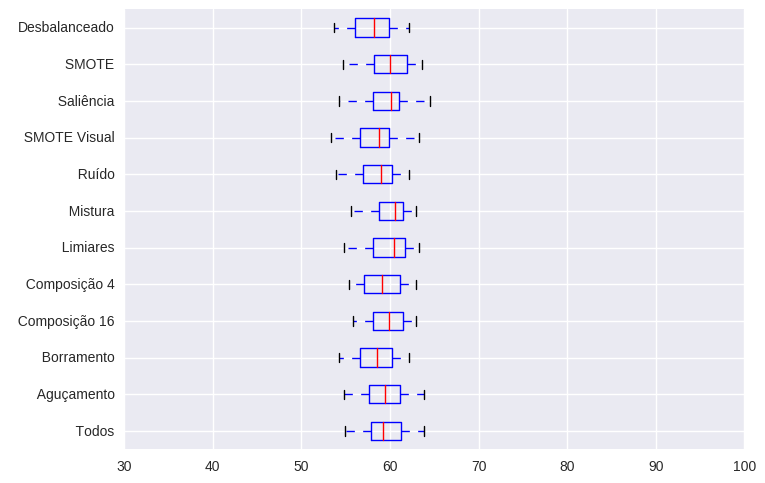
\includegraphics[width=\linewidth]{\detokenize{figuras/resultados/3/LBP_Luma_corel.png}}
  \end{center}
  \caption[Experimento com as 10 classes da base Corel. Foi utilizado o método Luma para conversão em escala de cinza e LBP como método de extração de características.]{Experimento com as 10 classes da base Corel. Foi utilizado o método Luma para conversão em escala de cinza e LBP como método de extração de características. \textit{Fonte:~Elaborado pela autora.}}
  \label{fig:resultados:3:melhor}
\end{figure}
\end{minipage}

\begin{table}[!htbp]
\centering
\caption{Resultados de \textit{f1-score} para as 10 classes da Corel, utilizando \emph{Luma} como método para conversão em escala de cinza e \emph{LBP} para extração de características}
\label{tab:resultados:3:melhor}
\begin{tabular}{|l|c|c|}
\hline
\textbf{Luma e LBP} & \textbf{Média} & \textbf{Desvio padrão} \\ \hline
Todos               & 59.46          & 2.23                   \\ \hline
Aguçamento          & 59.32          & 2.33                   \\ \hline
Borramento          & 58.41          & 2.36                   \\ \hline
Composição 16       & 59.71          & 1.92                   \\ \hline
Composição 4        & 58.97          & 2.20                   \\ \hline
Limiares            & 59.89          & 2.33                   \\ \hline
Mistura             & \textbf{59.99} & 2.02                   \\ \hline
Ruído               & 58.48          & 2.21                   \\ \hline
SMOTE Visual        & 58.43          & 2.35                   \\ \hline
Saliência           & 59.63          & 2.07                   \\ \hline
SMOTE               & 59.78          & 2.36                   \\ \hline
Desbalanceado       & 58.09          & 2.31                   \\ \hline
\end{tabular}
\end{table}

%-------------------------------------------------------------------------------
\item[] \textbf{Resultado da maior variância obtida com a combinação dos métodos de extração e conversão para escala de cinza}

\begin{minipage}{\linewidth}
  \begin{figure}[H]
    \begin{center}
        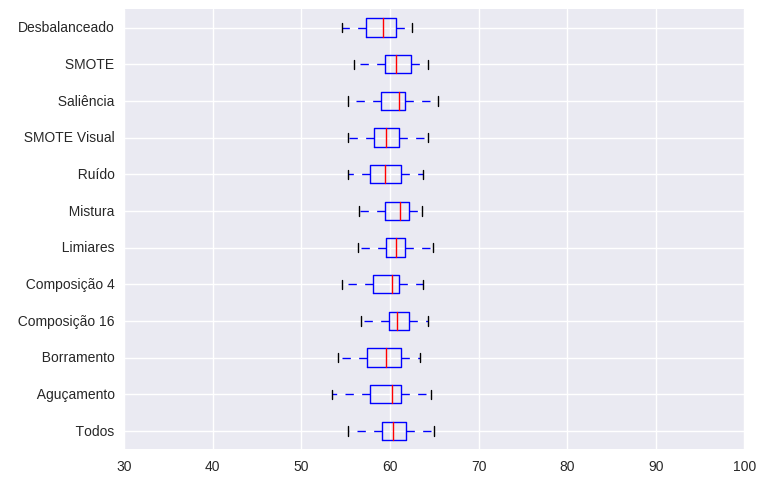
\includegraphics[width=\linewidth]{\detokenize{figuras/resultados/3/LBP_Intensity_corel.png}}
    \end{center}
    \caption[Experimento com as 10 classes da base Corel. Foi utilizado o método \emph{Intensidade} para conversão em escala de cinza e LBP como método de extração de características.]{Experimento com as 10 classes da base Corel. Foi utilizado o método \emph{Intensidade} para conversão em escala de cinza e LBP como método de extração de características. \textit{Fonte:~Elaborado pela autora.}}
    \label{fig:resultados:3:pior}
  \end{figure}
\end{minipage}

\begin{table}[]
\centering
\caption{Resultados de \textit{f1-score} para as 10 classes da Corel, utilizando \emph{Intensidade} como método para conversão em escala de cinza e \emph{LBP} para extração de características}
\label{tab:resultados:3:pior}
\begin{tabular}{|l|c|c|}
\hline
\textbf{LBP Intensity} & \textbf{Média}     & \textbf{Desvio Padrão} \\ \hline
Todos                  & 60.39          & 2.35               \\ \hline
Aguçamento             & 59.78          & 2.51               \\ \hline
Borramento             & 59.30          & 2.34               \\ \hline
Composição 16          & \textbf{60.73} & 2.23               \\ \hline
Composição 4           & 59.77          & 2.30               \\ \hline
Limiares               & 60.59          & 2.24               \\ \hline
Mistura                & 60.71          & 2.16               \\ \hline
Ruído                  & 59.39          & 2.44               \\ \hline
SMOTE Visual           & 59.44          & 2.26               \\ \hline
Saliência              & 60.36          & 2.18               \\ \hline
SMOTE                  & 60.49          & 2.22               \\ \hline
Desbalanceado          & 58.91          & 2.20               \\ \hline
\end{tabular}
\end{table}

%-------------------------------------------------------------------------------
\item[] \textbf{Discussão}

\end{itemize}

%%%%%%%%%%%%%%%%%%%%%%%%%%%%%%%%%%%%%%%%%%%%%%%%%%%%%%%%%%%%%%%%%%%%%%%%%%%%%%%%
\FloatBarrier
\subsection{Experimento 4: classes naturalmente desbalanceadas}

\begin{itemize}
%-------------------------------------------------------------------------------
\item[] \textbf{Base de Imagens}


%-------------------------------------------------------------------------------
\item[] \textbf{Protocolo}

O seguinte protocolo foi seguido para a obtenção dos resultados:

\begin{enumerate}
\item \textbf{Classes de imagens originais}:
\item \textbf{Desbalanceamento}:
\item \textbf{Método para geração artificial}:
\item \textbf{Quantização}:
\item \textbf{Extração de características}:
\item \textbf{Classificação}:
\end{enumerate}
%-------------------------------------------------------------------------------
\item[] \textbf{Resultados e Discussão}

\begin{figure}[!htbp]
  \begin{center}
      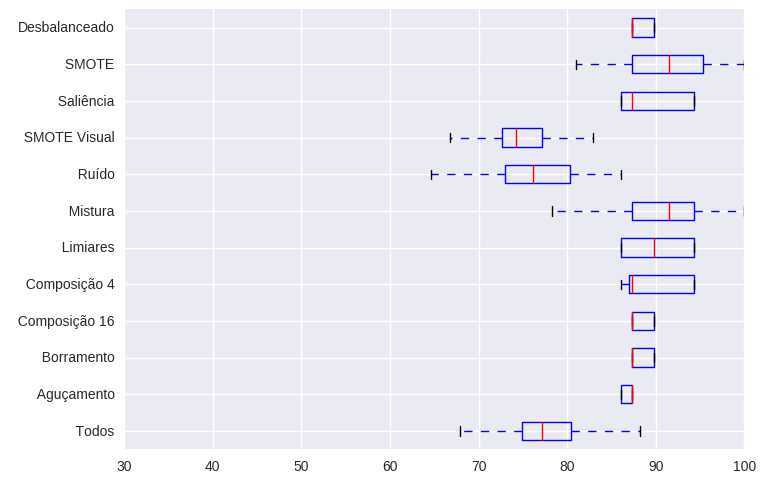
\includegraphics[width=\linewidth]{\detokenize{figuras/resultados/4/HOG_Luminance_eiffel-ponte.png}}
  \end{center}
  \caption[]{\textit{Fonte:~Elaborado pela autora.}}
  \label{fig:resultados:2:melhor}
\end{figure}

\begin{table}[]
\centering
\caption{Resultados de \textit{f1-score} para as classes XX, utilizando \emph{Luminância} como método para conversão em escala de cinza e \emph{HOG} para extração de características}
\label{tab:resultados:4:melhor}
\begin{tabular}{|l|c|c|}
\hline
\textbf{Luminância \& HOG} & \textbf{Média}     & \textbf{Desvio Padrão} \\ \hline
Todos                      & 77.373797          & 5.112180               \\ \hline
Aguçamento                 & 87.831980          & 7.039036               \\ \hline
Borramento                 & 85.051780          & 9.816291               \\ \hline
Composição 16              & 85.051780          & 9.816291               \\ \hline
Composição 4               & 85.392703          & 10.069356              \\ \hline
Limiares                   & 86.213200          & 10.528769              \\ \hline
Mistura                    & 90.312440          & 7.357446               \\ \hline
Ruído                      & 75.523828          & 6.209384               \\ \hline
SMOTE Visual               & 74.109795          & 4.093989               \\ \hline
Saliência                  & 85.713360          & 10.399830              \\ \hline
SMOTE                      & \textbf{90.711873} & 6.423170               \\ \hline
Desbalanceado              & 85.051780          & 9.816291               \\ \hline
\end{tabular}
\end{table}


\end{itemize}

%%%%%%%%%%%%%%%%%%%%%%%%%%%%%%%%%%%%%%%%%%%%%%%%%%%%%%%%%%%%%%%%%%%%%%%%%%%%%%%%
\FloatBarrier
\subsection{Experimento 5: classes com muitas imagens}

\begin{itemize}
%-------------------------------------------------------------------------------
\item[] \textbf{Base de Imagens}


%-------------------------------------------------------------------------------
\item[] \textbf{Protocolo}

O seguinte protocolo foi seguido para a obtenção dos resultados:

\begin{enumerate}
\item \textbf{Classes de imagens originais}:
\item \textbf{Desbalanceamento}:
\item \textbf{Método para geração artificial}:
\item \textbf{Quantização}:
\item \textbf{Extração de características}:
\item \textbf{Classificação}:
\end{enumerate}
%-------------------------------------------------------------------------------
%-------------------------------------------------------------------------------
\item[] \textbf{Resultado da melhor combinação dos métodos de extração e conversão para escala de cinza}

\begin{minipage}{\linewidth}
  \begin{figure}[H]
  \begin{center}
      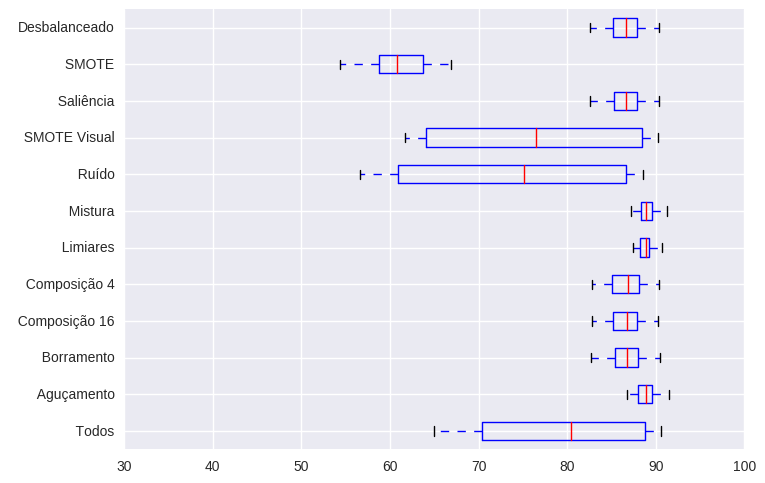
\includegraphics[width=\linewidth]{\detokenize{figuras/resultados/5/HOG_Gleam_deer-ship.png}}
  \end{center}
  \caption[]{\textit{Fonte:~Elaborado pela autora.}}
  \label{fig:resultados:5:melhor}
\end{figure}
\end{minipage}

\begin{table}[!htbp]
\centering
\caption{Resultados de \textit{f1-score} para as classes \emph{Tubarão} e \emph{Peixe}, utilizando \emph{Gleam} como método para conversão em escala de cinza e \emph{HOG} para extração de características}
\label{tab:resultados:5:melhor}
\begin{tabular}{|l|c|c|}
\hline
\textbf{Gleam e HOG} & \textbf{Média} & \textbf{Desvio padrão} \\ \hline
Todos                & 79.38          & 9.88                   \\ \hline
Aguçamento           & 88.88          & 1.13                   \\ \hline
Borramento           & 86.69          & 1.81                   \\ \hline
Composição 16        & 86.61          & 1.84                   \\ \hline
Composição 4         & 86.69          & 1.97                   \\ \hline
Limiares             & 88.93          & 1.04                   \\ \hline
Mistura              & \textbf{88.99} & 0.98                   \\ \hline
Ruído                & 73.72          & 13.18                  \\ \hline
SMOTE Visual         & 76.23          & 12.51                  \\ \hline
Saliência            & 86.61          & 1.86                   \\ \hline
SMOTE                & 60.90          & 3.46                   \\ \hline
Desbalanceado        & 86.60          & 1.86                   \\ \hline
\end{tabular}
\end{table}

\end{itemize}

%%%%%%%%%%%%%%%%%%%%%%%%%%%%%%%%%%%%%%%%%%%%%%%%%%%%%%%%%%%%%%%%%%%%%%%%%%%%%%%%
% \begin{figure}[!htbp]
%   \begin{center}
%     \begin{subfigure}{.49\linewidth}
%       \centering
%       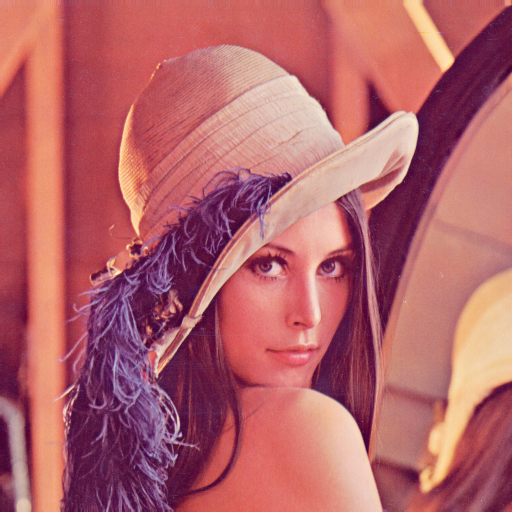
\includegraphics[width=\linewidth]{\detokenize{figuras/visualizacao/original.png}}
%     \end{subfigure}
%     \begin{subfigure}{.49\linewidth}
%       \centering
%       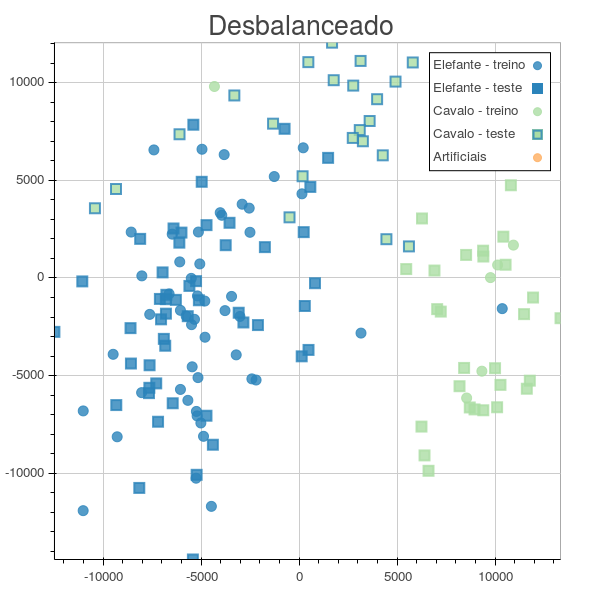
\includegraphics[width=\linewidth]{\detokenize{figuras/visualizacao/desbalanceado-fixed.png}}
%     \end{subfigure}
%   \end{center}
%   \caption{Remoção de 50\% das imagens de treino da classe Cavalo.}
%   \label{fig:desbalanceado}
% \end{figure}

%-------------------------------------------------------------------------------

% Também foi possível notar que algumas operações não provocaram a melhora da classificação. A operação de adição de ruído para geração artificial, a posterior extração utilizando CCV e a quantização por MSB, destacou-se como o pior resultado, apresentado na Figura~\ref{fig:resultpior}. Outros casos que não obtiveram o resultado esperado envolveram as operações de borramento e de \textit{unsharp masking}.

% Após a realização dos testes, as operações que melhor se destacaram foram: utilizar todas as operações, apenas mistura e apenas composição. E as operações que resultaram em uma classificação pior do que o uso do SMOTE foram: utilizar apenas borramento, ruído ou \textit{unsharp masking}. Com o teste estatístico de Friedman foi possível verificar que o ACC foi o extrator que melhor se beneficiou das características geradas; e CCV e GCH os menos beneficiados. \enlargethispage{-\baselineskip} A Tabela \ref{tab:result} apresenta os \textit{rankings} encontrados por este teste para todas as execuções das melhores operações. O p-valor computado corresponde a $4.24E^{-11}$, assim a hipótese nula de que não há diferença entre as execuções foi rejeitada. Vale destacar que para algumas execuções, o teste de Friedman retornou o \textit{ranking}: geração artificial (1), SMOTE (2) e imagens originais (3), ou seja, sem que SMOTE e a geração artificial concorressem pela mesma posição, diferente da tabela apresentada.
%
% \begin{table}[htb]
% \centering
% \caption{Posição média dos algoritmos utilizando Friedman}
%   \begin{tabular}{c|c}
%     Algoritmos  &   Posição \\ \hline
%     Original    &   3.0000  \\
%     Smote       &   1.6136  \\
%     Artificial  &   1.3863  \\
%   \end{tabular}
%  \label{tab:result}
% \end{table}
%
% Em outro experimento, utilizou-se as cópias das imagens de treino para rebalancear, sem realizar nenhuma operação de pré-processamento (método conhecido como SRS - \textit{Simple Random Sampling}). A Figura~\ref{fig:resultcopia} mostra as respectivas medidas-F encontradas. É possível notar que a cópia dessas imagens não adiciona nenhuma informação nova para o aprendizado.
%
% \begin{figure}[htb]
%  \begin{center}
%    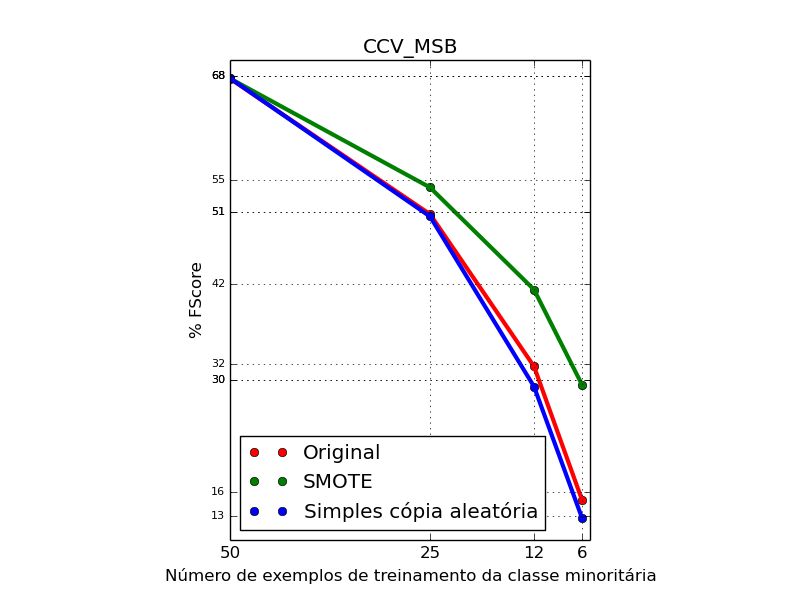
\includegraphics[width=\linewidth]{\detokenize {figuras/resultado-copia.png}}
%  \end{center}
%   \caption[Simples replicação de exemplos sem realizar nenhuma operação.]{Simples replicação de exemplos sem realizar nenhuma operação de pré-processamento. É possível verificar que não foi adicionada nenhuma informação relevante para o aprendizado. \textit{Fonte:~Elaborado pela autora.}}
%  \label{fig:resultcopia}
% \end{figure}
%
%
\section{Considerações Finais}

Este estudo apresentou evidências experimentais de que, em problemas de duas classes, pode haver ganho estatístico do \textit{f-score} ao gerar imagens, quando comparado à geração de exemplos artificiais no espaço de atributos (ou seja, depois que as características já foram extraídas das imagens).  Com os experimentos realizados foi possível notar que a geração de imagens artificiais pode gerar novas informações para a classificação das imagens. O que indica que um estudo aprofundado de cada contexto pode relatar quais operações podem ser aplicadas nas imagens originais de forma a auxiliar o cenário de bases desbalanceadas.
